\documentclass[11pt, compress,tikz]{beamer}

\usepackage{preamb}
\graphicspath{{./../doc/_images/}}
\usepackage{minted}
\usemintedstyle{monokai}
\definecolor{backmonokai}{HTML}{282828}
\setminted{bgcolor=backmonokai} 
%%%%%%%%%%%%%%%%%%%%%%%%%%%%%%%%%% Styling for the beamer %%%%%%%%%%%%%%%%%%%%%%%%%%%%%%%%
%%%%%%%%%%%%%%%%%%%%%%%%%%%%%%%%%%%%%%%%%%%%%%%%%%%%%%%%%%%%%%%%%%%%%%%%%%%%%%%%%%%%%%%%%%

\setbeamertemplate{navigation symbols}{} 
\usetheme{Warsaw}

\setbeamertemplate{theorem begin}{{
\inserttheoremheadfont
\inserttheoremname
\inserttheorempunctuation
}}

\setbeamertemplate{theorem end}{}
\newtheorem{proposition}[theorem]{Proposition}

\theoremstyle{definition}
\newtheorem{mydef}[theorem]{Définition}
\makeatletter

%\captionsetup[figure]{labelformat=empty}
\definecolor{beamer@blendedpurp}{rgb}{0.41, 0.16, 0.38}
 % 0.8,0.2,0.3 rouge carmin presque rose assez élégant avec rgb
 %235 77 77 corail
 % .75 ,.2,.2 rouge clair 
\setbeamercolor{structure}{fg=beamer@blendedpurp}
\setbeamercolor*{palette quaternary}{fg=black,bg=white!80!gray } %bg=couleur à gauche header back
\makeatother
%\setbeamercolor{section in head/foot}{} no touch en fait casse tout
%\setbeamercolor{subsection in head/foot}{fg=black,bg=gray!30} idem 

\makeatletter
\defbeamertemplate*{footline}{shadow theme}
{%
  \leavevmode%
  \hbox{\begin{beamercolorbox}[wd=.5\paperwidth,ht=2.5ex,dp=1.125ex,leftskip=.3cm,rightskip=.3cm plus1fil]{title in head/foot}%
    \usebeamerfont{title in head/foot}\insertshorttitle%
  \end{beamercolorbox}}%
  \begin{beamercolorbox}[wd=.5\paperwidth,ht=2.5ex,dp=1.125ex,leftskip=.3cm plus1fil,rightskip=.3cm]{author in head/foot}%
    \usebeamerfont{author in head/foot}\hfill\insertframenumber\,/\,\inserttotalframenumber
  \end{beamercolorbox}%
  \vskip0pt%
}

%\setbeamertemplate{section in toc}{\textcolor{structure.fg}{$\blacktriangleright$}\hspace{1.2 em}~\inserttocsection \\}

%\setbeamertemplate{section in toc}{\inserttocsectionnumber.~\inserttocsection}
\setbeamercolor*{section in toc}{fg=black}
\setbeamercolor*{enumerate item}{fg=black}
\setbeamercolor*{enumerate subitem}{fg=black}
\newcommand*{\rom}[1]{\expandafter\@slowromancap\romannumeral #1@}
\makeatother

%%%%%%%%%%%%%%%%%%%%%%%%%%%%%%%%%%%%%%%%%%%%%%%%%%%%%%%%%%%%%%%%%%%%%%%%%%%%%%%%%
%%%%%%%%%%%%%%%%%%%%%%%%%%%%%%%%%% end styling beamer %%%%%%%%%%%%%%%%%%%%%%%%%%%
\usepackage{tcolorbox}
\newtcolorbox{mybox}{colback=red!5!white,colframe=red!75!black}


\title{Package chaoseverywhere}
\subtitle{Software development HMMA238}
\author{\vspace*{-1.5cm}Lefort Tanguy, Coiffier Ophélie and Gaizi Ibrahim}
\date{\vspace*{-2cm}06-2020}
\institute[Montpellier University]{University of Montpellier}
\titlegraphic{%
  \makebox[0.9\paperwidth]{%
    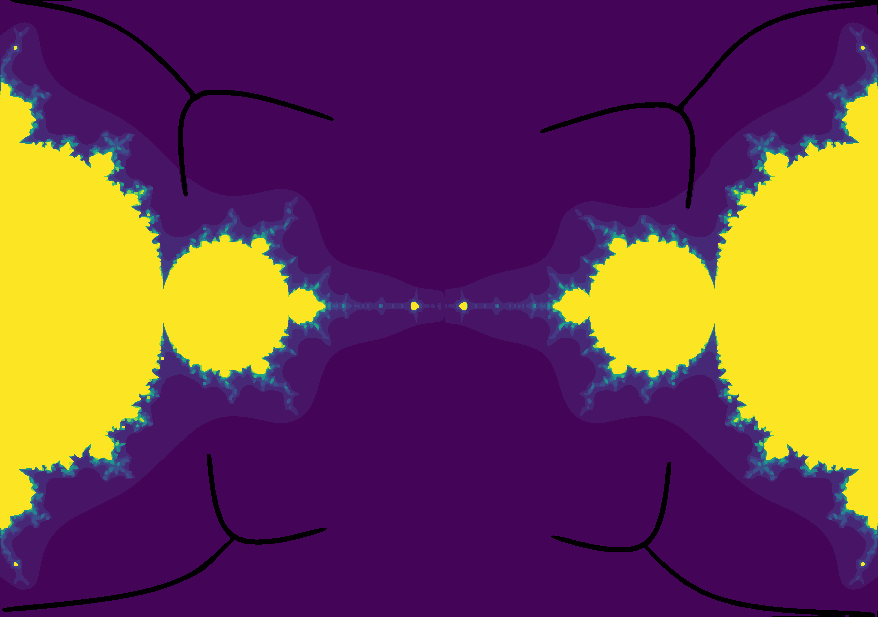
\includegraphics[scale=.2]{logo1_f.pdf}%
    \hfill%
    
\includegraphics[scale=.1]{logo_univ.pdf}%
    \hspace{.25cm}
  }%
}

\begin{document}

{
\def\mytitleframe{\bgroup
\makeatletter
\setbeamertemplate{footline}
{%
  \leavevmode%
  \hbox{\begin{beamercolorbox}[wd=.5\paperwidth,ht=2.5ex,dp=1.125ex,leftskip=.3cm,rightskip=.3cm plus1fil]{title in head/foot}%
    \usebeamerfont{title in head/foot}\insertshorttitle%
  \end{beamercolorbox}}%
  \begin{beamercolorbox}[wd=.5\paperwidth,ht=2.5ex,dp=1.125ex,leftskip=.3cm plus1fil,rightskip=.3cm]{author in head/foot}%
    \usebeamerfont{author in head/foot}%\hfill\insertframenumber\,/\,\inserttotalframenumber
  \end{beamercolorbox}%
  \vskip0pt%
}
\maketitle
\egroup
\addtocounter{framenumber}{-1}
}
\makeatother
	\mytitleframe
}


\section*{Contents}
\setbeamertemplate{background}{%
   \tikz\node[opacity=0.2] at (current page.center) {
   					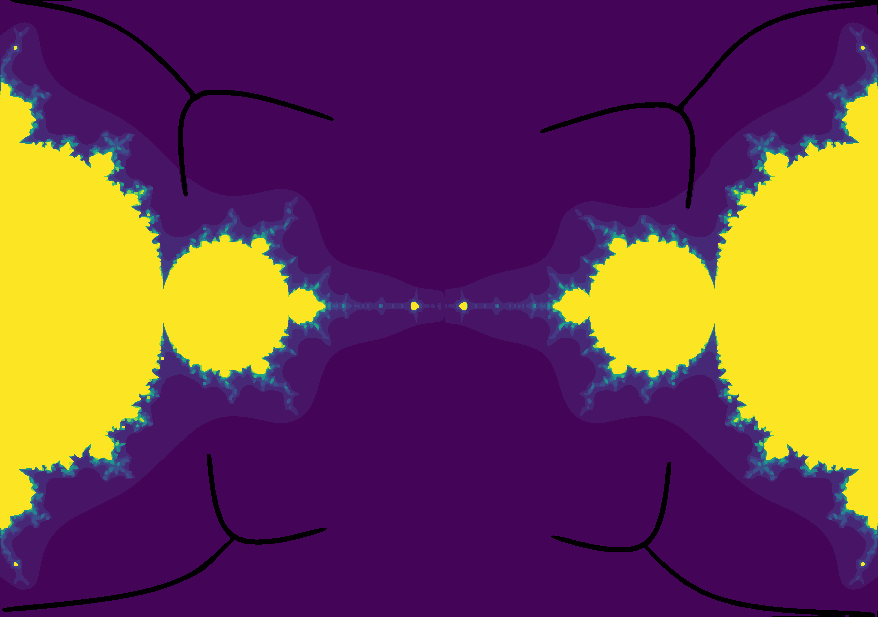
\includegraphics[trim = 1.1cm 0cm 0cm 0cm]{logo1_f.pdf}};}
\begin{frame}
\frametitle{Table of contents}
  \tableofcontents
\end{frame}      
\setbeamertemplate{background}{}


\section{Chaoseverywhere}
\subsection{Introduction}
\begin{frame}[fragile]{Chaoseverywhere}
Python3 package : \textit{\textbf{Chaoseverywhere}}%
\begin{minted}{python}
>>> import chaoseverywhere as chaos
\end{minted}
Includes $2$ main themes:
\begin{enumerate}[label=$\bullet$]
    \item the Manldebrot set,  %
    \item the logistic map. %
\end{enumerate}
\begin{block}<2>{Specific dependencies}
\begin{enumerate}[label=\ding{51}]
\item FFMPEG
\item Mayavi
\end{enumerate}
\end{block}
\end{frame}

\subsection{Generalities}
\begin{frame}[fragile]{Generalities}
Our subject deals with fractals and the chaos theory.
\begin{description}
   \item [Fractal :] has an object that has at least one of the following characteristics:
    \begin{enumerate}[label=$\bullet$]
        \item a self-similarity at different scale,
        \item self-similar structures can be observed within the figure,
        \item the Haussdorff dimension isn't an integer.
    \end{enumerate}
    \item [Chaos :] is study of the patterns one can find in a system that seems totally random.
\end{description}
\end{frame}

\section[Logistic map]{The logistic map}
\subsection{The map}

\begin{frame}[fragile]{The logistic map: the cobweb diagram}
\vspace{-.25cm}
\begin{block}{Map formula}
\[x_{n+1} = rx_{n}(1-x_{n})\]
\end{block}
\vspace{-.3cm}
\begin{onlyenv}<3>
\begin{minted}{python}
>>> chaos.logistic_draw(x0=0.01, r=3.6, 50, 100)
\end{minted}
\end{onlyenv}
\begin{columns}
          \column{0.60\linewidth}
             \begin{onlyenv}<1-3>
             \vspace{-1.2cm}
  \begin{center}
    \includegraphics<3>[clip,scale=0.5, trim={.5cm 0 1.5cm 1.5cm}]{logistic_cobweb.pdf}
  \end{center}
\end{onlyenv}
             
           \column{0.40\linewidth}
           \vspace{-1.2cm}
           \begin{enumerate}[label=$\bullet$]
               \item<1-> $1 < r \leq 3 $: one point of convergence
               \item<2-> $3 < r \leq 3.57$ : oscillations between several values
               \item<3-> $r > 3.57$ : chaotic behavior
           \end{enumerate}
         \end{columns} 
\end{frame}

\subsection{Bifurcation diagram}
\begin{frame}{Bifurcation diagram}
A summary of the logistic map : the bifurcation diagram
\begin{center}
    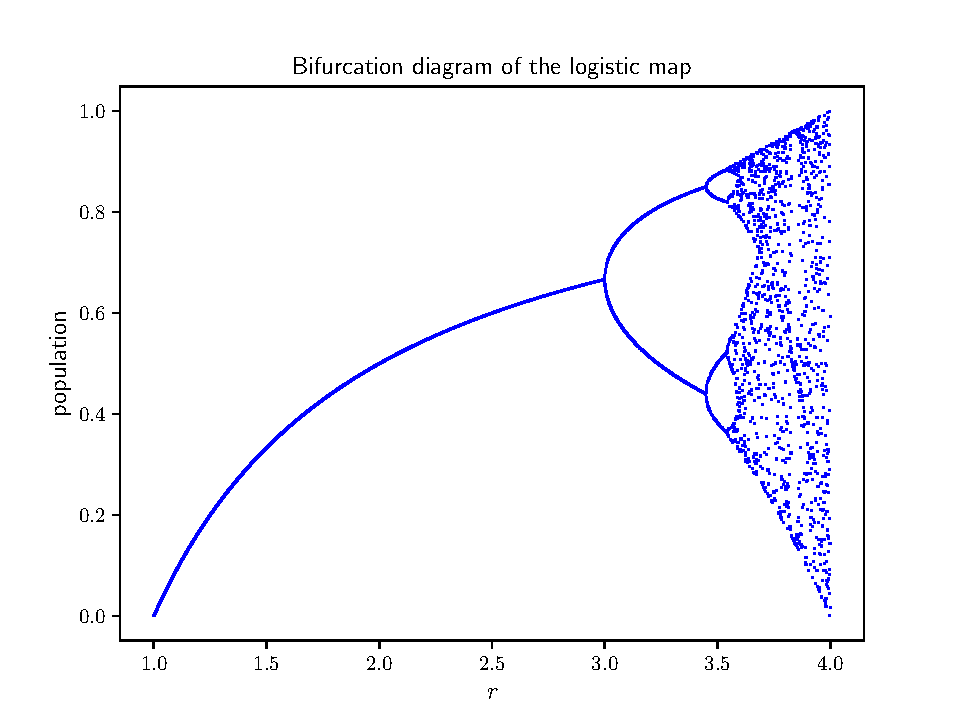
\includegraphics[scale=0.6]{bifurcation.pdf}
\end{center}
\end{frame}



\section[Mandelbrot]{The Mandelbrot set}
\subsection{Definition and caracteristics}
\begin{frame}{The Mandelbrot set: definition}

\begin{block}{Definition}
The Mandelbrot set $\mathcal{M}$ is:
$$\mathcal{M}=\left\{ c\in\mathbb{C},\ (z_n)_n \text{ is bounded},\ \text{with } z_{n+1}=z_n^2+c,\ z_0=0\right\}.$$
\end{block}

\end{frame}

\subsection{Visualization}
\begin{frame}{\emph{Mandel\_loop } function}
The code on one side, the figure on the other, or above, or below


\begin{center}
    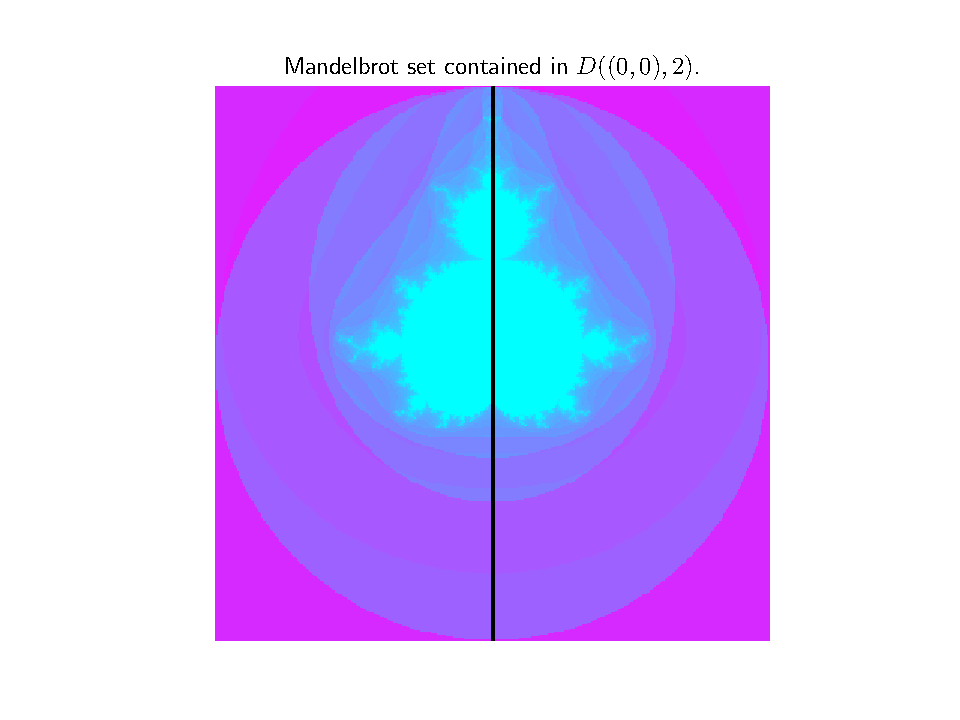
\includegraphics[scale=0.55]{mandelbrot.pdf}
\end{center}
\end{frame}




\section[Link]{Mandelbrot set and bifurcation diagram}

\begin{frame}
\frametitle{Link between Mandelbrot set and bifurcation diagram}
If you're unable to display the animation, click here:
\href{https://www.youtube.com/watch?v=xYQbqML1eE4}{\beamergotobutton{Youtube}}

\IfFileExists{./img_connections/les_3-1.pdf}{\begin{figure}
					\animategraphics[controls,width=\linewidth,
					height=6cm,keepaspectratio]{30}{./img_connections/les_3-}{1}{360}
     				\end{figure}
     					}{\begin{center}
     						\begin{mybox}
     						\centering
     						\Large{Please click on the link above to see one \\
     													 wonderful animation!}
     						\end{mybox}
						\end{center}     				
     					}

\end{frame}

\section[]{Conclusion}
\begin{frame}{Conclusion}
Conclusion
\end{frame}      

\end{document}